\section{Анализ требований к программному средству и разработка функциональных требований}
\label{sec:domain}

\subsection{Функциональная модель программного средства}
\label{sec:domain:model}

Функциональная модель программного средства представлена в виде\linebreakсхемы алгоритма процесса обучения и диаграммы вариантов использования и информационной модели предметной области. Варианты использования отражают функциональность системы в ответ на внешние воздействия с точки зрения получения значимого результата для пользователей. Информационная модель предметной области в дальнейшем будет использоваться при проектировании базы данных для программного средства.

%\subsubsection{} Анализ процесса образования
%\label{sec:domain:model:deeds}

%Перед началом проектирования необходимо проанализировать процесса образования. В связи с отсутствием опыта преподавания у исполнителя данного дипломного проекта выглядит целесообразным проведение данного анализа с точки зрения студента. Результат анализа представлен в виде схемы алгоритма на рисунках \ref{fig:domain:model:deeds:student_algorithm} и \ref{fig:domain:model:deeds:student_algorithm_2}. Схема ограничивается процессом обучения в семестре и не включает проверку знаний в виде зачетов и экзаменов, завершающих обучение по дисциплине.

%Одной из особенностей данной схемы является цикличность, с которой выполняется процесс обучения. Цикл начинается изучением некоторой теории по дисциплине, затем на практическом или лабораторном занятии преподаватель разъясняет некоторые сложные моменты, которые могут возникнуть при выполнении индивидуальных заданий, выдаёт условие заданий, а также вариант. Студент на занятии или дома выполняет задание. После этого на одном из занятий или вне их происходит защита результатов выполнения заданий. После этого происходит оценивание результатов преподавателем. Если задание выполнено не полностью, то оно отправляется на доработку. Если же оценка не является удовлетворительной, то преподаватель вправе выдать новое задание.

%Таким образом на схеме алгоритма приведен типичный вариант обучения студента, который широко практикуется в университетах и практически никак не автоматизирован. Программное средство, разработка которой ведется в данном дипломном проекте, не изменит устоявшейся системы сразу, однако значительно упростит выполнение многих ее этапов.

\subsubsection{} Варианты использования программного средства
\label{sec:domain:model:use_cases}

В результат анализа предметной области и существующих аналогов можно сделать вывод, что проектируемое программное средство должно поддерживать набор функций, который бы полностью удовлетворял потребности пользователей с точки зрения обычной социальной сети, а также специфические функции, необходимые только для мотоцикслистов. Выделим следующие:

\begin{itemize}
	\item \emph{Интеграция с существуюшими социальными сетями}, которая позволит производить авторизацию в приложении с использованием существующих учетных записей пользователей из других социальных сетей.
	\item \emph{Сообщения} позволяют обмениваться информацией, находить друзей и единомышленников.
	\item \emph{Публикации} представляют собой записи, которые могут содержать фото, видеофайлы и текст записи с хештегами.
	\item \emph{Управления мотопарком}. Возможность прикрепления информации о мотопарке пользователя: создание публикаций с указанием технических характеристик мотоциклов, а также удаление и редактирование данной информации.
	\item \emph{Гараж}. Страница отображает информацию о мотопарке пользователя: фотографии, видео, технические характеристики, комментарии других пользователей, лайки. 
	\item \emph{Профиль пользователя}. Отдельная страница, которая отображает краткую информацию о человеке, его мотопарке, а также содержит секцию с публикациями пользователя.
	\item \emph{Личный блог}. Возможность ведения личного блога предусматривает создание публикаций с пометкой <<Запись>>. Данные публикации будут отмечены специальным индефикатором в секции со всеми публикациями (профиль пользователя).
	\item \emph{Управление друзьями и подписчиками}. Возможность отправки и отмены запросов на добавления в друзья, поиск других пользователей.
	\item \emph{Отправка оповещений}. Возможность отправки оповещений о состоянии приложения, а также о действиях других пользователей (комментирование публикакации, добавление лайков на запись).
	\item \emph{Настройка учетной записи} позволит изменять информацию о пользователе, прикреплять ссылки на другие социальные сети, устанавливать настройки приватности, изменять пароль.
	\item \emph{Лента}. Отдельная страница, которая представляет собой список публикаций. Следует предусмотреть ее разграничение на публикации, размещенные только друзьями, и на популярные, которые получили больше всего лайков в приложении.
	\item \emph{Режим катания на мотоцикле}. Возможность переключения в данный режим указывет на то, что пользователь в данный момент едет на мотоцикле или изъявляет желание покататься.
	\item \emph{Карта}. Отдельный раздел приложения, который представляет собой страницу, содержащую карту с геолокацией, на которой отмечены друзья, у которых установлен режим катания на мотоцикле, а также метки. Следует предусмотреть функцию возврата фокуса к текущему местоположению, а также поиск друзей.
	\item \emph{Метки}. Специальные маркеры на карте, которые будут служить инструментом предупреждения других пользователей об опаснастях и чрезвычайных ситуациях на дороге.
	\item \emph{Маячок}. Возможность отправки специального сигнала в виде текстового сообщения другу, который в данный момент катается на мотоцикле, т.е. отмечен на карте.
	%которые отображаются на карте, бывают двух типов: <<Предупреждение>> и <<SOS>>. При установке последнего пользователем его друзьям должно приходить оповещение с оповещение должно приходить 
\end{itemize}

Диаграмма вариантов использования, разработанная с использованием нотации \uml, представлена на рисунке~\ref{fig:domain:model:use_cases:model}.
Рассмотрим некоторые из представленных на рисунке прецедентов.

\begin{figure}[H]
\centering
	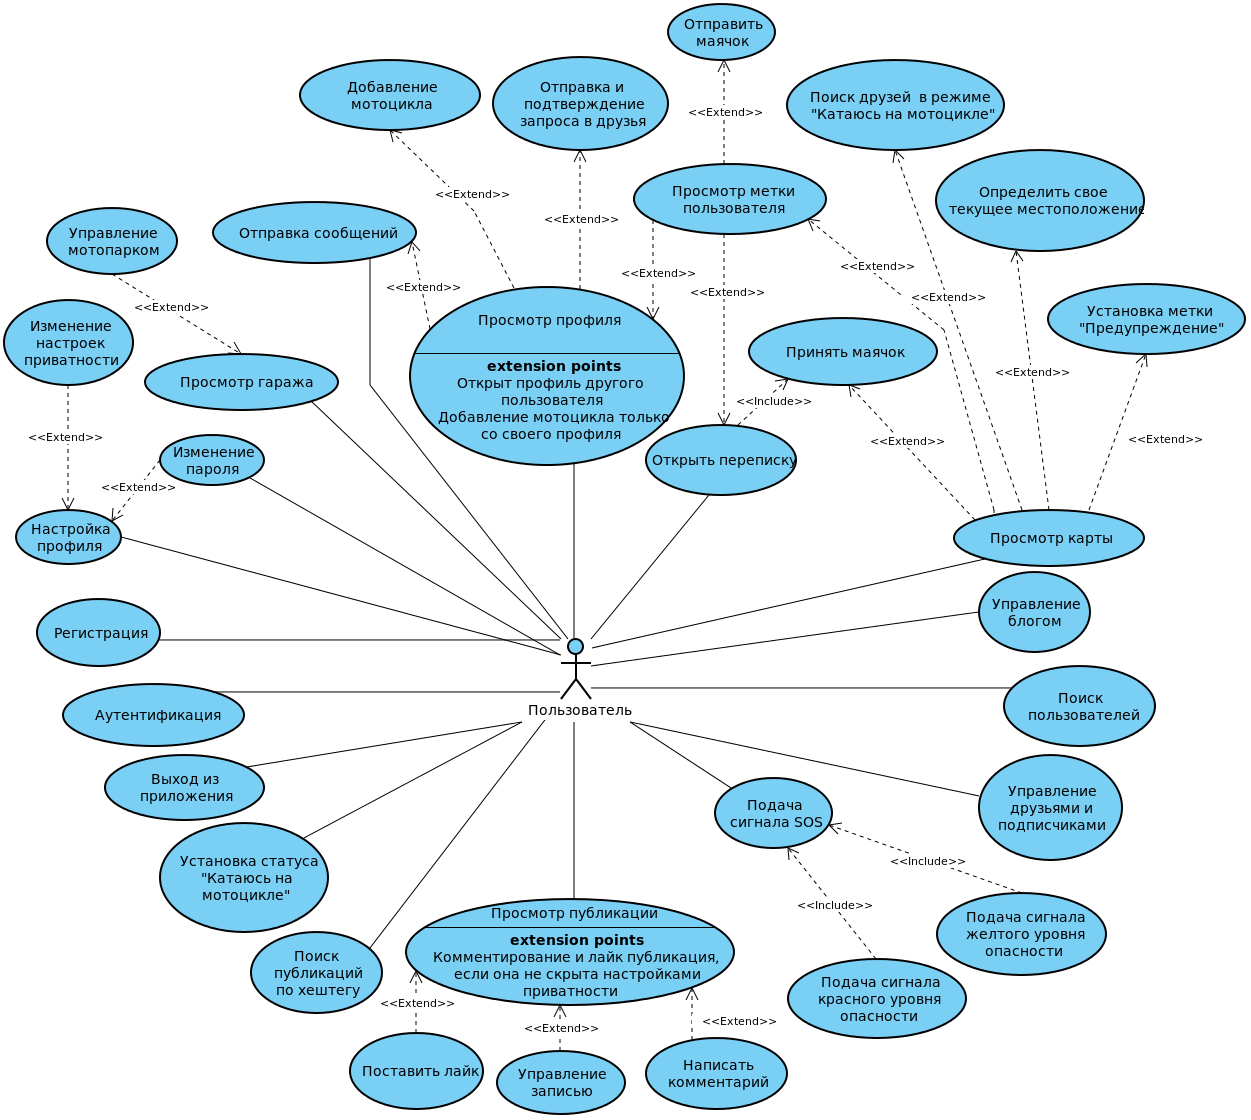
\includegraphics[height=230mm, width=155mm]{use-case-diagram.png}
	\caption{Диаграмма вариантов использования ПС}
	\label{fig:domain:model:use_cases:model}
\end{figure}

\emph{Регистрация, аутентификация и авторизация}. В приложения планируется реализация собственной системы авторизации, а также возможность регистрации с помощью учетных записей от других социальных сетей (\facebook~и \vk.).
Важно предусмотреть возможность редактирование информации о пользователе, в том числе и его учетных данных (н.п. \emph{смена пароля}). Для этих целей будет создан специальный раздел с \emph{настройками профиля}.
Также следует предусмотреть возможность смены пароля со страницы входа в приложение, т.к. пользователь может забыть пароль.
Важной функцией приложения станет \emph{изменение настроек приватности}, что даст возможность ограничить видимость информации о себе и публикакаций от других пользователей. 

\subsection{Разработка спецификации функциональных требований}
\label{sec:domain:specification}

С учетом требований, определенных в подразделе \ref{sec:analysis:specification}, представим детализацию функций проектируемого ПС.

\subsubsection{} Функция регистрации
\label{sec:domain:specification:signup}

Функция регистрации должна быть реализована с учетом следующих требований:
\begin{itemize}
	\item для регистрации пользователь обязан предоставить номер мобильного телефона и пароль;
	\item возможность альтернативной регистрации с помощью социальных сетей <<ВКонтакте>> и Facebook;
	\item проверка номера мобильного телефона проверяется отправкой SMS-сообщения с кодом подверждения;
	\item хранение пароля в хешированном виде; алгоритм шифрования должен превосходить или быть равным семейству SHA-2. Использование соли обязательно;
	\item предусмотреть возможность смены пароля после регистрации путем отправки SMS-сообщение с кодом, ввод которого перенаправляет на страницу изменения пароля.
\end{itemize}

\subsubsection{} Функция аутентификации
\label{sec:domain:specification:authentication}

Функция аутентификации должна быть реализована с учетом следующих требований:
\begin{itemize}
	\item инициатором является пользователь, при этом необходимо предоставить номер мобильного телефона и пароль, либо выбрать вход через Facebook или <<ВКонтакте>>;
	\item должна быть реализована возможность повторной аутентификации пользователя без необходимости ввода какой-либо информации;
	\item возможность восстановления пароля.
\end{itemize}

Для восстановления пароля пользователь должен предоставить номер мобильного телефона. На предоставленный номер высылается SMS-сообщение с кодом подверждения. После ввода отправленного кода ему предоставляется возможность установить новый пароль.

\subsubsection{} Функция управления публикациями
\label{sec:domain:specification:agenda}

Публикации являются главной единицой обмена информацией в социальной сети. При реализации данной функции необходимо учесть следующие требования:
\begin{itemize}
	\item необходимо обеспечить возможность добавления, удаления, редактирования публикации;
	\item публикация может включать в себя текст, фото или видео;
	\item для ведения личного блога создать отдельный раздел <<Записи>>; все публикации, созданные в данном разделе, будут относится к блогу пользователя;
	\item записи с личного блога должны быть помечены специальным идентификатором в галлерее публикаций профиля пользователя;
	\item должна быть реализована возможность загрузки фото и видео как с галерии мобильного телефона, так и с его камеры;
	\item предусмотреть возможность указания хештегов в тексте, что облегчит поиск нужных публикаций в ленте;
	\item добавить возможность наложения цветовых фильтров на фотографии, как в социальной сети Instagram;
	\item предусмотреть возможность комментирования и лайка публикации с отображением количества лайков и всей истории комментариев;
	\item при нажатии на количество лайков появляется список всех лайкнувших пользователей через который можно перейти к ним в профиль.
	\item при нажатии на публикацию она должна открываться на отдельной странице (галлерия профиля, гараж, лента).
\end{itemize}

\subsubsection{} Функция управления мотопарком
\label{sec:domain:specification:subjects}

Функция управления мотопарком должна быть реализована с учетом следующих требований:
\begin{itemize}
	\item мотоцикл представляет собой обычную публикацию с дополнительной возможностью прикрепления нескольких фото и видеозаписей. Описание публикации в данном случае --- характеристики мотоцикла;
	\item характеристики мотоцикла представить следующими полями: производитель, модель, прозвище, модификация, год, цвет, пробег, объем двигателя, мощность, описание;
	\item предоставить возможность добавления, редактирования, измения записей о мотоциклах;
	\item все добавленные мотоциклы формирует страницу <<Гараж>>, которая представляет собой список всех прикрепленных мототоциклов.
\end{itemize}

\subsubsection{} Функция обмена сообщениями
\label{sec:domain:specification:messages}

Функция коммуникации должна реализовывать следующие требования:
\begin{itemize}
	\item должна быть возможность отправки сообщений одного пользователя другому;
	\item история сообщений представляется в виде диалогов, где отображается текст сообщения, имя пользователя и время отправки сообщения;
	\item возможность прикрепления фотографии к сообщению (с галерии или с камеры телефона);
	\item предоставить возможность удаления выбранного диалога, а также поиска нужного.
\end{itemize}

\subsubsection{} Функция просмотра профиля пользователя
\label{sec:domain:specification:student_history}

Следующая группа требований относится к профилю пользователя:
\begin{itemize}
	\item профиль пользователя состоит из следующих секциий: аватар, информация о пользователе (количество мотосезонов и т.д.) и мотоциклах, количество друзей, подписчиков, подписок, записей, галлерея публикаций;
	\item предоставить возможность добавления новой публикации и прикрепления мотоцикла со страницы профиля;
	\item должна быть возможность отправки запроса в друзья при переходе в профиль другого пользователя;
	\item при переходе в профиль друга добавить возможность  перенаправления на страницу с диалогом;
\end{itemize}

\subsubsection{} Функция просмотра ленты
\label{sec:domain:specification:student_history}

Функция просмотра ленты должна реализовывать следующие требования:
\begin{itemize}
	\item лента представляет собой отдельную страницу со списком публикаций и полем поиска;
	\item поиск осуществляется по хештегам, указанным в тексте описания публикации;
	\item предоставить возможность разделения списка публикаций на 2 вида: принадлежащие друзьям и популярные (по количеству лайков).
\end{itemize}

\subsubsection{} Функция просмотра ленты
\label{sec:domain:specification:student_history}

Функция просмотра ленты должна реализовывать следующие требования:
\begin{itemize}
	\item лента представляет собой отдельную страницу со списком публикаций и полем поиска;
	\item поиск осуществляется по хештегам, указанным в тексте описания публикации;
	\item предоставить возможность разделения списка публикаций на 2 вида: принадлежащие друзьям и популярные (по количеству лайков).
\end{itemize}

\subsubsection{} Функция подачи сигнала SOS
\label{sec:domain:specification:student_history}

Следующая группа требований относится к установке сигнала SOS:
\begin{itemize}
	\item создать отдельный раздел в навигации приложения для установки сигнала;
	\item сигнал SOS должен отображаться в виде метки на карте;
	
	\item метка SOS устанавливается только в случае ДТП;
	
	\item сигнал должен иметь разделение на уровень тревоги: красный и желтый;
	\item красный сигнал подается только при опасности для здоровья;
	\item каждая метка, которая отображает сигнал, должна быть окрашена в соответствующий уровню тревоги цвет;
	\item при отправке пользователем сигнала красного уровня всем его друзья должно приходить push-уведомление.
\end{itemize}

\subsubsection{} Функция просмотра карты
\label{sec:domain:specification:student_history}

Функция просмотра карты должна реализовывать следующие требования:
\begin{itemize}
	\item карта представляет собой раздел геолокации, на котором отображаются метки следующих типов: друзья в режиме <<Катаюсь на мотоцикле>> (отображается в виде аватара), метки предупреждений и сигналов SOS;
	\item при нажатии на метку предупреждения или сигнала SOS на карте должно появляться ее текстовое описание;
	\item при установке метки предупреждения обязательно нужно указать ее текстовое описание;
	\item предусмотреть возможность опредения своего текущего местоположения;
	\item добавить отдельную кнопку для уставноки метки предупреждения;
	\item предусмотреть возможность поиска друзей, которые катаются на мотоцикле в данный момент врмени.
\end{itemize}

\subsubsection{} Функция отправки маячка
\label{sec:domain:specification:student_history}

Функция отправки маячка должна реализовывать следующие требования:
\begin{itemize}
	\item для отправки маячка следует перейти в карту приложения и выбрать нужного пользователя;
	\item по нажатию на метку пользователя должно появляться всплывающее окно, содержащее поле ввода маячка, а также кнопки перехода в диалог и профиль;
	\item адресату маячка должно приходить push-уведомление на телефон, а также сообщение в диалог с отправителем;
	\item принять маячок можно перейдя в диалог с отправителем, нажав кнопку <<Принять маячок>>;
	\item если у адресата в момент отправления откыта карта, то должно появляться всплывающее окно, в котором также можно его принять;
\end{itemize}

\subsubsection{} Функция управления друзьями и подписчиками
\label{sec:domain:specification:student_history}

Функция управления друзьями и подписчиками должна реализовывать следующие требования:
\begin{itemize}
	\item предусмотреть создание отдельного раздела <<Друзья>>, который разделен на 3 секции: друзья, запросы, подписки;
	\item секция состоит из списка соответсвующих пользоватателей и 2-ух счетчиков: первый отображает общее количество, а 2-ой количество находящихся в сети;
	\item релизовать возможности отправки и принятия запроса в друзья, а также удаление из друзей;
	\item при отправке запроса дружбы пользователю также отправляется соответсвующее push-уведомление.
	\item для подписки на другого пользователя достаточно отправить запрос в друзья, при этом данный пользователь будет отображен в секции подписок;
	\item запросы в дружбу, отправленные пользователю, можно посмотреть в секции запросов;
	\item если один пользователь удаляет другого, то у первого второй переносится в подписчики, а у второго первый в подписки соответственно;
	\item первый пользователь может вернуть второго в друзья перейдя в секцию запросов.
\end{itemize}

\subsubsection{} Разработка инфологической модели базы данных
\label{sec:domain:model:db}

Исходя из необходимости использования в проектируемом приложении базы данных, разработаем ее инфологическую модель. Диаграмма, представляющая модель базы данных инфологического уровня~\cite{kulikov_db_workbook}, представлена на рисунке~\ref{fig:domain:model:db:model}.

\begin{figure}[H]
\centering
	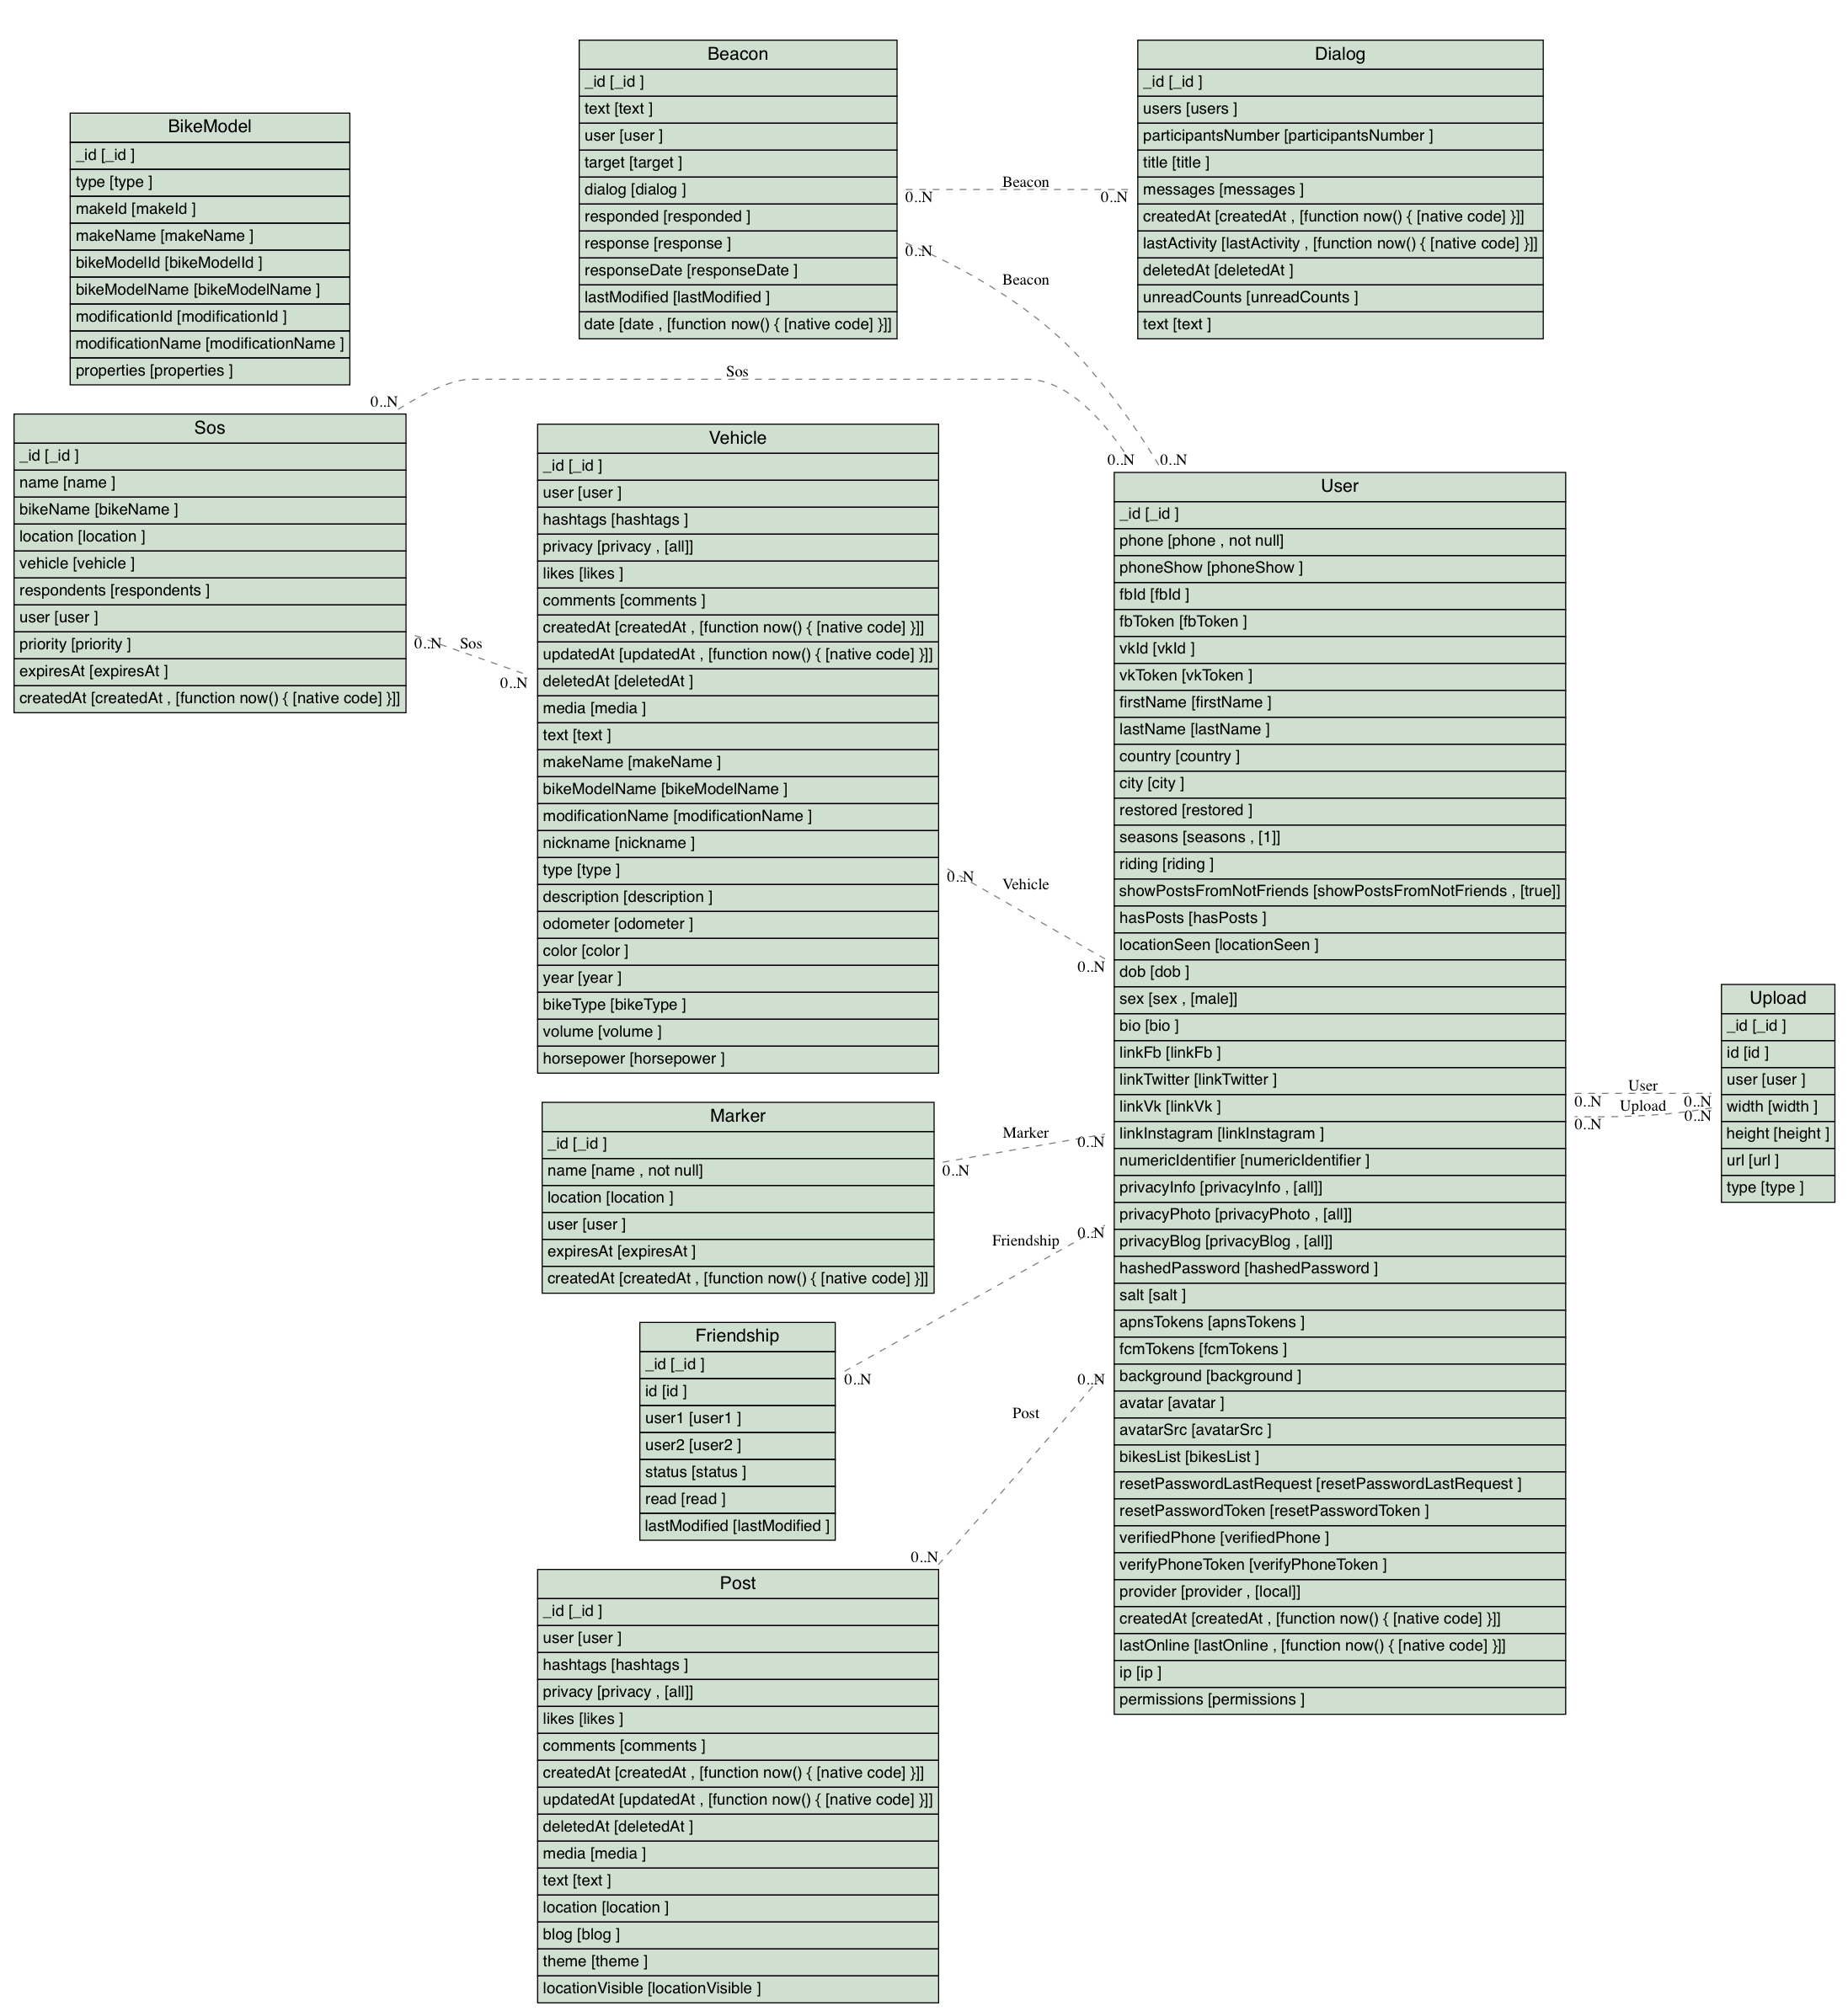
\includegraphics[scale=0.2]{erd.png}
	\caption{Инфологическая модель базы данных}
	\label{fig:domain:model:db:model}
\end{figure}

Важно отметить, что модель BikeModel используется для генирования набора существующих мотоциклов на стадии запуска серверного приложения. Это необходимо для удобного добавления мотоцикла из списка существующих, который представлен моделью Vehile. Информация о возможных мотоциклах сожержится на серверной части.

В информационной модели предусмотрены возможности для обеспечения безопасности аутентификации и авторизации: в модели User предусмотрены поля для хранения хешированного пароля и соли, а также токены от социальных сетей Facebook и <<ВКонтакте>>.

Метки сигалов SOS и предупреждения представлены моделью Marker. Важно отметить, что данная модель содержит даты создания маркера и его пропажи. Это сделано для того, чтобы не отображать огромное количество меток на карте. После прохождения определенного промежутка времени, заданного на сервере, они пропадают.

Сигнал SOS представлен отдельной моделью, содержит набор пользователей, которые откликнулись на сигнал помощи, приоритет: желтый или красный.

Функция переписки реализована с помощью модели Dialog, cодержит количество непрочитанных сообщений, количество участников диаога (на данный момент поддерживается только 2).















